\documentclass[11pt,a4paper]{article}
\usepackage[margin=24mm]{geometry}
\usepackage{amsmath,amssymb,booktabs,graphicx,float,tikz}
\usepackage[hidelinks]{hyperref}
\usepackage[T1]{fontenc}
\usetikzlibrary{positioning,arrows.meta}
\setlength{\parskip}{5pt}
\setlength{\parindent}{0pt}
\setlength{\emergencystretch}{2em}
\title{Assignment 2: Cost-Efficient Segmentation under a Compute Budget}
\author{Jatin Purbia --- B23CH1022\\CSL7360 --- Computer Vision\\Indian Institute of Technology Jodhpur}
\date{29 October 2026}
\begin{document}
\maketitle
\begin{abstract}
This project implements Track B using original lightweight fully convolutional networks trained from scratch. It shares one preprocessing and inference implementation across prediction, evaluation and timing, and computes the prescribed metrics manually. Experimental claims are limited to saved evidence. The results table explicitly identifies missing evaluations; authentic personal photographs and their annotations cannot be replaced by synthetic evidence. This document is an implementation report until all required experiments and photographs are present.
\end{abstract}

\section{Introduction}
The task is binary salient-object segmentation: assign each pixel to the main object(s) or background without interactive object selection. The objective is to maximize the prescribed Cost-Efficient Segmentation (CES) score subject to a mean single-thread CPU inference budget of 50 milliseconds. Region overlap alone is insufficient: the quality term also rewards accurate boundaries. Three small encoder--decoder designs explore standard, deeper and depthwise separable convolutions. No pretrained model or parameters are used.

\section{Dataset and leakage prevention}
DUTS contains 10,553 training photographs (DUTS-TR) and 5,019 test photographs (DUTS-TE)~\cite{duts}. A sorted list of DUTS-TR stems is shuffled using Python's seed-42 random generator; round$(0.1N)$ IDs form validation. For the official training size this gives 9,498 training and 1,055 validation IDs. The actual manifests, once prepared, are saved and hashed. Intel(R) Core(TM) 7 150U. Actual saved split: 9498 training and 1055 validation images; seed 42.

All architecture, loss, threshold, resolution and stopping decisions use only DUTS-TR validation. The experiment runner never loads DUTS-TE. Final evaluation requires a frozen parameter-file hash and records all 5,019 samples individually. Personal photos are testing-only and require 5--10 authentic phone captures covering at least three condition categories. A script can validate files and author attestations; it cannot prove photographic authenticity or scene diversity.

\section{Preprocessing}
OpenCV reads BGR uint8 photographs. Every original photo is directly resized to $256\times256$ using \texttt{INTER\_AREA}; aspect ratio is intentionally squashed. Grayscale masks use \texttt{INTER\_NEAREST} and are binarized at intensity 128 inclusive. The network receives RGB float32 tensors $[B,3,H,W]$ in $[0,1]$, with no mean/std normalization. Training augmentation jointly flips image/mask horizontally with probability $0.5$ and applies brightness/contrast multipliers sampled uniformly in $[0.9,1.1]$ to images only. Validation and test preprocessing are deterministic.

The timed pipeline starts after the original resize. It includes BGR-to-RGB conversion, tensor creation, normalization, optional bilinear downscaling, forward inference, bilinear upsampling of logits to $256\times256$, sigmoid, thresholding and conversion to a binary uint8 array. Masks on disk are multiplied by 255 after timing.

\section{Proposed architectures}
The default three-stage Tiny FCN uses widths $(b,2b,4b)$. Each encoder block is Conv--BatchNorm--ReLU; max pooling halves spatial size between blocks. The decoder bilinearly upsamples to each skip's size, concatenates encoder features and applies a new convolution block. A $1\times1$ head produces a single logit channel. The U-Net candidate adds a second convolution in each encoder stage. The separable candidate replaces each block with a depthwise spatial convolution followed by a pointwise projection, each normalized and activated. These designs were written using permitted PyTorch layers rather than importing a model architecture.

\begin{figure}[htbp]\centering
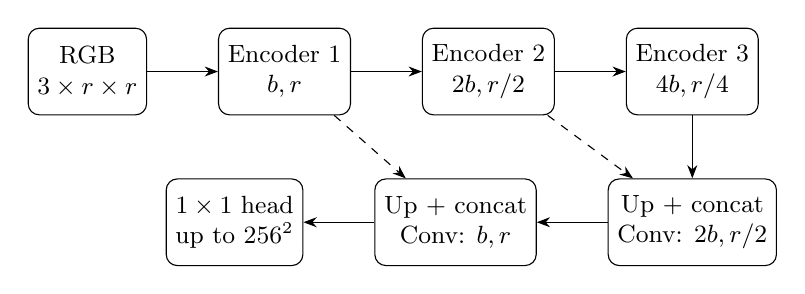
\begin{tikzpicture}[node distance=8mm and 9mm, box/.style={draw,rounded corners,align=center,font=\small,minimum height=11mm}, >=Stealth]
\node[box] (in) {RGB\\$3\times r\times r$};
\node[box,right=of in] (e1) {Encoder 1\\$b,r$};
\node[box,right=of e1] (e2) {Encoder 2\\$2b,r/2$};
\node[box,right=of e2] (e3) {Encoder 3\\$4b,r/4$};
\node[box,below=of e3] (d2) {Up + concat\\Conv: $2b,r/2$};
\node[box,left=of d2] (d1) {Up + concat\\Conv: $b,r$};
\node[box,left=of d1] (out) {$1\times1$ head\\up to $256^2$};
\draw[->] (in)--(e1); \draw[->] (e1)--(e2); \draw[->] (e2)--(e3);
\draw[->] (e3)--(d2); \draw[->] (d2)--(d1); \draw[->] (d1)--(out);
\draw[->,dashed] (e2)--(d2); \draw[->,dashed] (e1)--(d1);
\end{tikzpicture}
\caption{Actual three-stage Tiny FCN topology. $r$ is internal resolution; $b$ is base width. Dashed arrows are concatenation skips. The chosen configuration and parameter count must be read from the frozen run, not inferred from this generic diagram.}
\end{figure}

Depth, base width, decoder width, kernel size, skip usage, and bilinear versus transpose upsampling are configurable. Untrained parameter/latency diagnostics are recorded separately from quality experiments. Fewer parameters do not establish lower measured latency.
Validation-selected candidate: unet16\_bce\_128\_infer96. Architecture: \{'kind': 'unet', 'base': 16, 'depth': 4\}; learned parameters: 439393; inference resolution: 96; threshold: 0.5.

\section{Mathematical formulation}
For input channel $c$, output channel $o$ and spatial offsets $(u,v)$, convolution is
\begin{equation}
z_{oij}=a_o+\sum_c\sum_u\sum_v W_{ocuv}x_{c,i+u,j+v}.
\end{equation}
Here $W$ contains learned filters and $a$ is a bias (omitted in normalized blocks). For logit $z_i$, probability $p_i$ and binary label $y_i$,
\begin{align}
p_i&=\sigma(z_i)=\frac{1}{1+e^{-z_i}}, & \hat y_i&=\mathbf1[p_i\ge\tau],\\
L_{\rm BCE}&=-\frac1N\sum_i\big[y_i\log p_i+(1-y_i)\log(1-p_i)\big],\\
L_{\rm Dice}&=1-\frac{2\sum_i p_iy_i+\epsilon}{\sum_i p_i+\sum_i y_i+\epsilon}, & \epsilon&=10^{-6},\\
L&=L_{\rm BCE}+\beta L_{\rm Dice}.
\end{align}
BCE is computed through the stable logits formulation. Dice is computed separately for each image and averaged. The default decision threshold is $\tau=0.5$; any change must use validation only. The mandatory baseline has $\beta=0$.

Aggregate all pixels in the evaluated dataset into
\begin{equation}
C=\begin{pmatrix}TN&FP\\FN&TP\end{pmatrix},\qquad
TP=\sum_i\mathbf1[\hat y_i=1,y_i=1],
\end{equation}
with analogous definitions for true negatives, false positives and false negatives. Rows denote true class; columns denote predicted class. Then
\begin{align}
\operatorname{IoU}_{fg}&=\frac{TP}{TP+FP+FN}, &
\operatorname{IoU}_{bg}&=\frac{TN}{TN+FP+FN},\\
\operatorname{mIoU}&=\tfrac12(\operatorname{IoU}_{fg}+\operatorname{IoU}_{bg}).
\end{align}
We assign an absent class (zero union) IoU of 1, representing correct absence. This is an explicit implementation convention because the PDF does not define that degeneracy. Per-image IoUs are never averaged to form the dataset score.

For foreground set $M$ and four-connected neighborhood $\mathcal N_4$,
\begin{equation}
\partial M=\{i\in M:\exists j\in\mathcal N_4(i),\; j\notin M\}.
\end{equation}
Pixels outside the image are background. Let $B_p=\partial\hat M$, $B_t=\partial M$, and $D_2(B)$ be pixels within a centered $5\times5$ window of $B$. Matching tolerance is Chebyshev distance two, including diagonal offsets $(2,2)$. For one image,
\begin{align}
P&=\frac{|B_p\cap D_2(B_t)|}{|B_p|}, & R&=\frac{|B_t\cap D_2(B_p)|}{|B_t|},\\
F_1&=\begin{cases}2PR/(P+R)&P+R>0,\\0&\text{otherwise},\end{cases} &
BF1&=\frac1K\sum_{k=1}^K F_{1,k}.
\end{align}
Both empty boundaries yield $F_1=1$; exactly one empty boundary yields $F_1=0$. Four directional tensor slices extract the boundary. Neighborhood matching uses 25 whole-array boolean OR passes over zero-padded NumPy views, with no per-pixel Python loop or library morphology. Analytic corner/diagonal tests and equivalence checks against the permitted \texttt{max\_pool2d} building block verify the exact window. Matching is many-to-many, as specified, rather than bipartite assignment. This optimization accelerates evaluation; metrics remain outside the inference timer.

For all quality metrics on the $[0,1]$ scale,
\begin{align}
Q&=0.70\operatorname{mIoU}+0.30BF1,\\
CES&=\begin{cases}
Q\left[1-0.20\frac{T_{CPU}}{50}-0.10\min\left(1,\frac{S_{disk}}{4194304}\right)\right],&T_{CPU}\le50,\\
0,&T_{CPU}>50.
\end{cases}
\end{align}
$T_{CPU}$ is in milliseconds and $S_{disk}$ is the actual parameter-file size in bytes. For $Q=.7$, $T=20$ and $S=524288$, the exact result is $.63525$, consistent with the PDF's rounded $.635$.

\section{Training methodology}
The baseline configuration uses AdamW, learning rate $10^{-3}$, weight decay $10^{-4}$, cosine scheduling over 40 epochs, batch size 8, patience 8 and gradient norm clipping at 5. The explicitly limited CPU pilot configuration uses two epochs, batch size 16 and smaller widths at resolution 128. These are different experiment budgets and must be identified when interpreting results. Every run saves its complete configuration, package versions, manifest hashes, best epoch, best validation metrics and per-epoch CSV logs. Best epoch selection maximizes validation $Q$ within each training run. Across candidates, final selection maximizes measured validation CES. Training checkpoints include optimizer and scheduler states; inference exports retain all learned weights and batch-normalization buffers.

The bounded refinement increases base width to 8 and encoder depth to four, with a four-epoch budget at training resolution 128. It is motivated by weak pilot boundary quality and low-resolution latency headroom. Capacity, context and training duration change together, so this is a practical refinement rather than a causal depth-only ablation. The full 40-epoch grid is supplied as configuration and is not claimed executed. Best-epoch training validation uses threshold $0.5$; inference resolution and the final threshold are then selected on the same DUTS-TR validation set. Test sets remain isolated until freeze.

\section{Computational efficiency and timing}
The encoder operates at a configurable internal resolution; the full output remains $256\times256$. Standard blocks prioritize simple CPU kernels, while separable blocks reduce arithmetic at the possible cost of additional operator overhead. Single-thread execution is configured before NumPy, OpenCV or PyTorch imports through four required environment variables, followed by their thread-setting APIs. Inference uses CPU tensors, \texttt{eval()} and \texttt{inference\_mode()}. No inference subprocess, data-loader worker or alternate engine is used.

One full warmup is excluded. For official timing, each DUTS-TE photo is loaded and resized outside the timer. The exact shared inference function is wrapped by \texttt{time.process\_time()}. The sum of all 5,019 durations divided by 5,019 gives $T_{CPU}$. Metrics and file exports occur outside timing. The prediction CLI instead uses its output-producing pass as warmup, then averages 20 additional full-pipeline runs. Size uses \texttt{os.path.getsize}; plain \texttt{torch.save} is not post-compressed.

\section{Experimental comparison}
The planned comparison isolates architecture, BCE versus BCE+Dice, and internal resolution. \texttt{results/model\_comparison.csv} contains only measured DUTS-TR validation scores. The selected row is saved with its checkpoint provenance before either final test set is opened. Synthetic fixtures verify software behavior; synthetic latency diagnostics do not establish DUTS segmentation quality or official timing compliance. Validation CES is an estimate for selection, while only the complete DUTS-TE CES is official.
\IfFileExists{../results/figures/q_vs_time.png}{\begin{figure}[htbp]\centering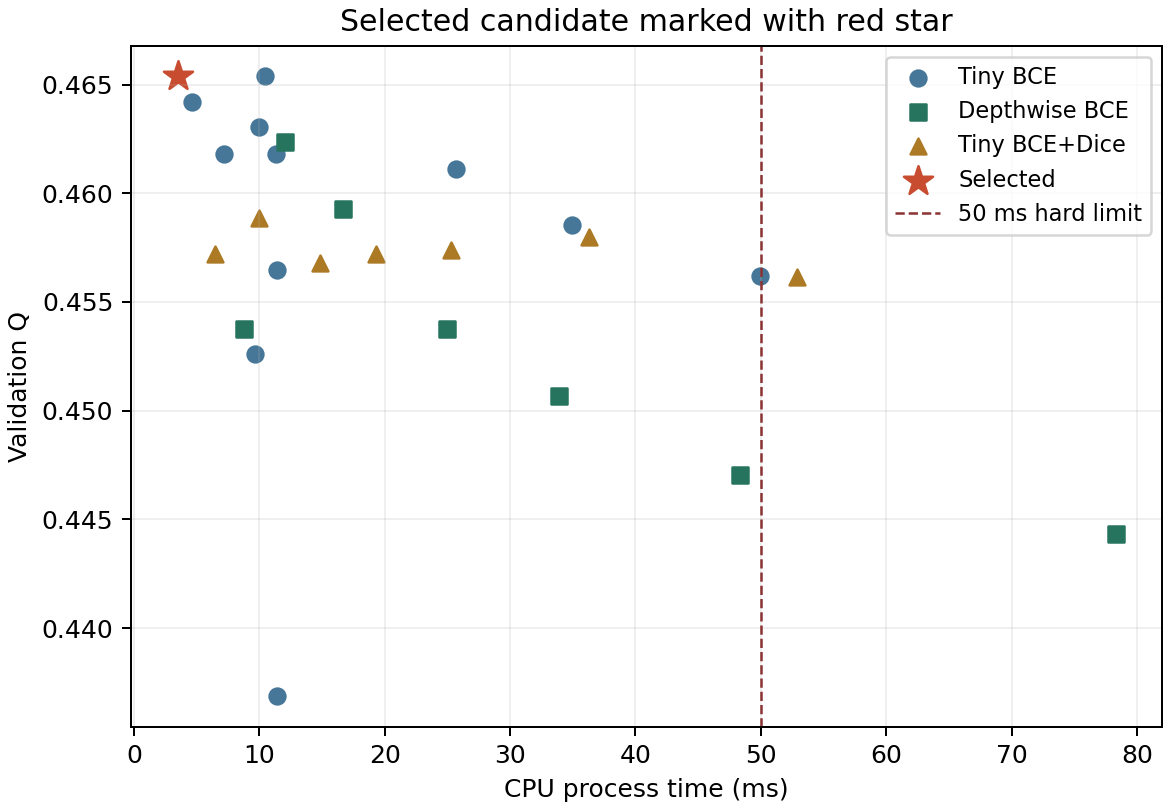
\includegraphics[width=.9\linewidth]{../results/figures/q_vs_time.png}\caption{Measured validation quality versus complete CPU pipeline time. Each point is an observed configuration; the red star marks selection. Full configuration names appear in the CES comparison.}\end{figure}}{}
\IfFileExists{../results/figures/size_vs_q.png}{\begin{figure}[htbp]\centering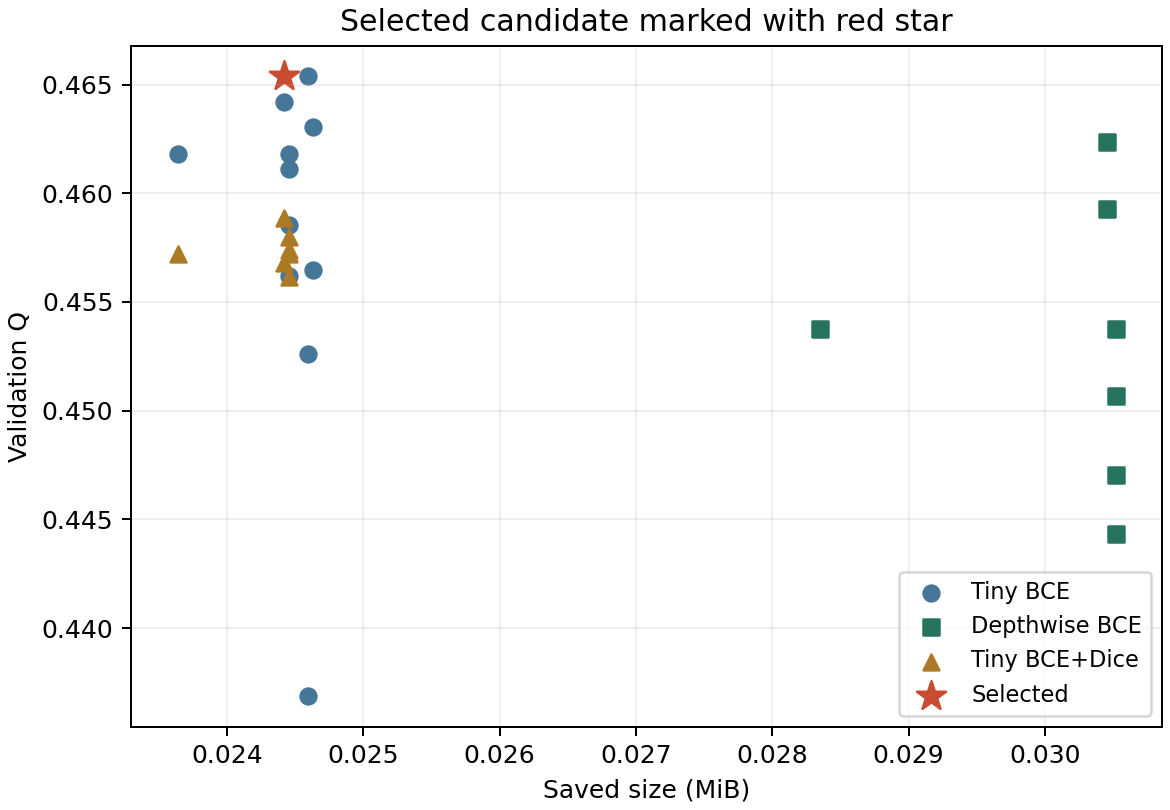
\includegraphics[width=.9\linewidth]{../results/figures/size_vs_q.png}\caption{Measured validation quality versus actual saved parameter size. Markers identify architecture/loss groups and the selected configuration.}\end{figure}}{}
\IfFileExists{../results/figures/ces_comparison.png}{\begin{figure}[htbp]\centering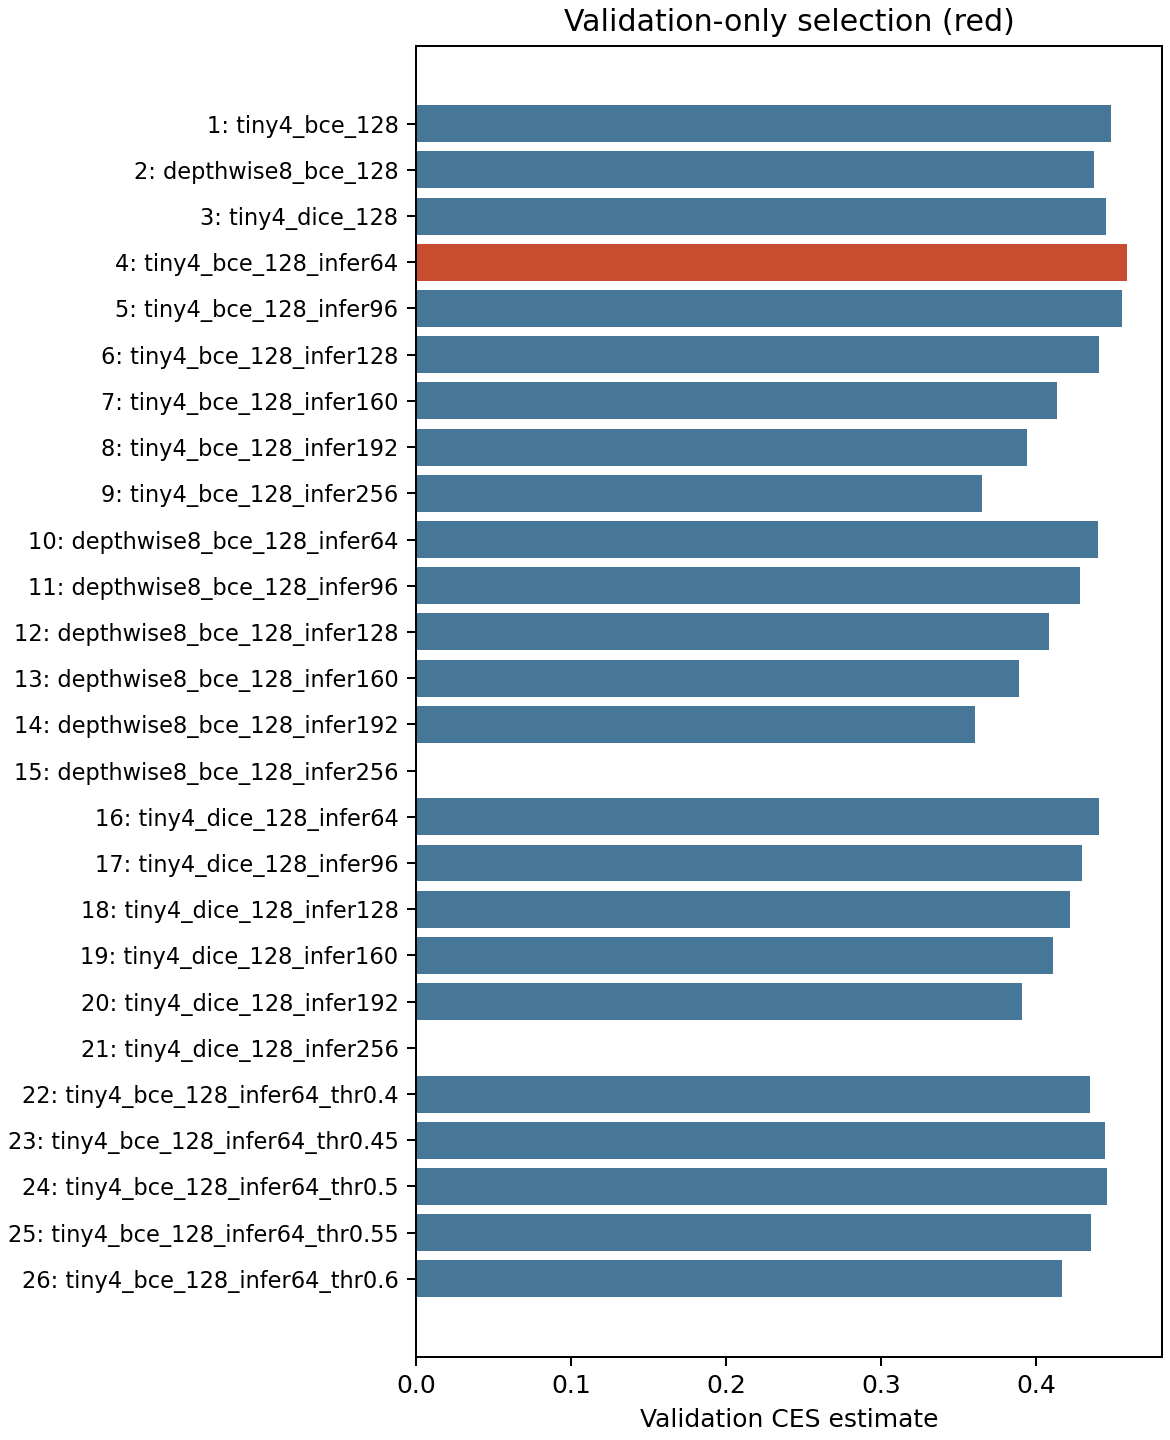
\includegraphics[width=.95\linewidth]{../results/figures/ces_comparison.png}\caption{Measured validation CES estimates and full candidate names. The selected configuration is red.}\end{figure}}{}
\IfFileExists{../results/figures/training.png}{\begin{figure}[htbp]\centering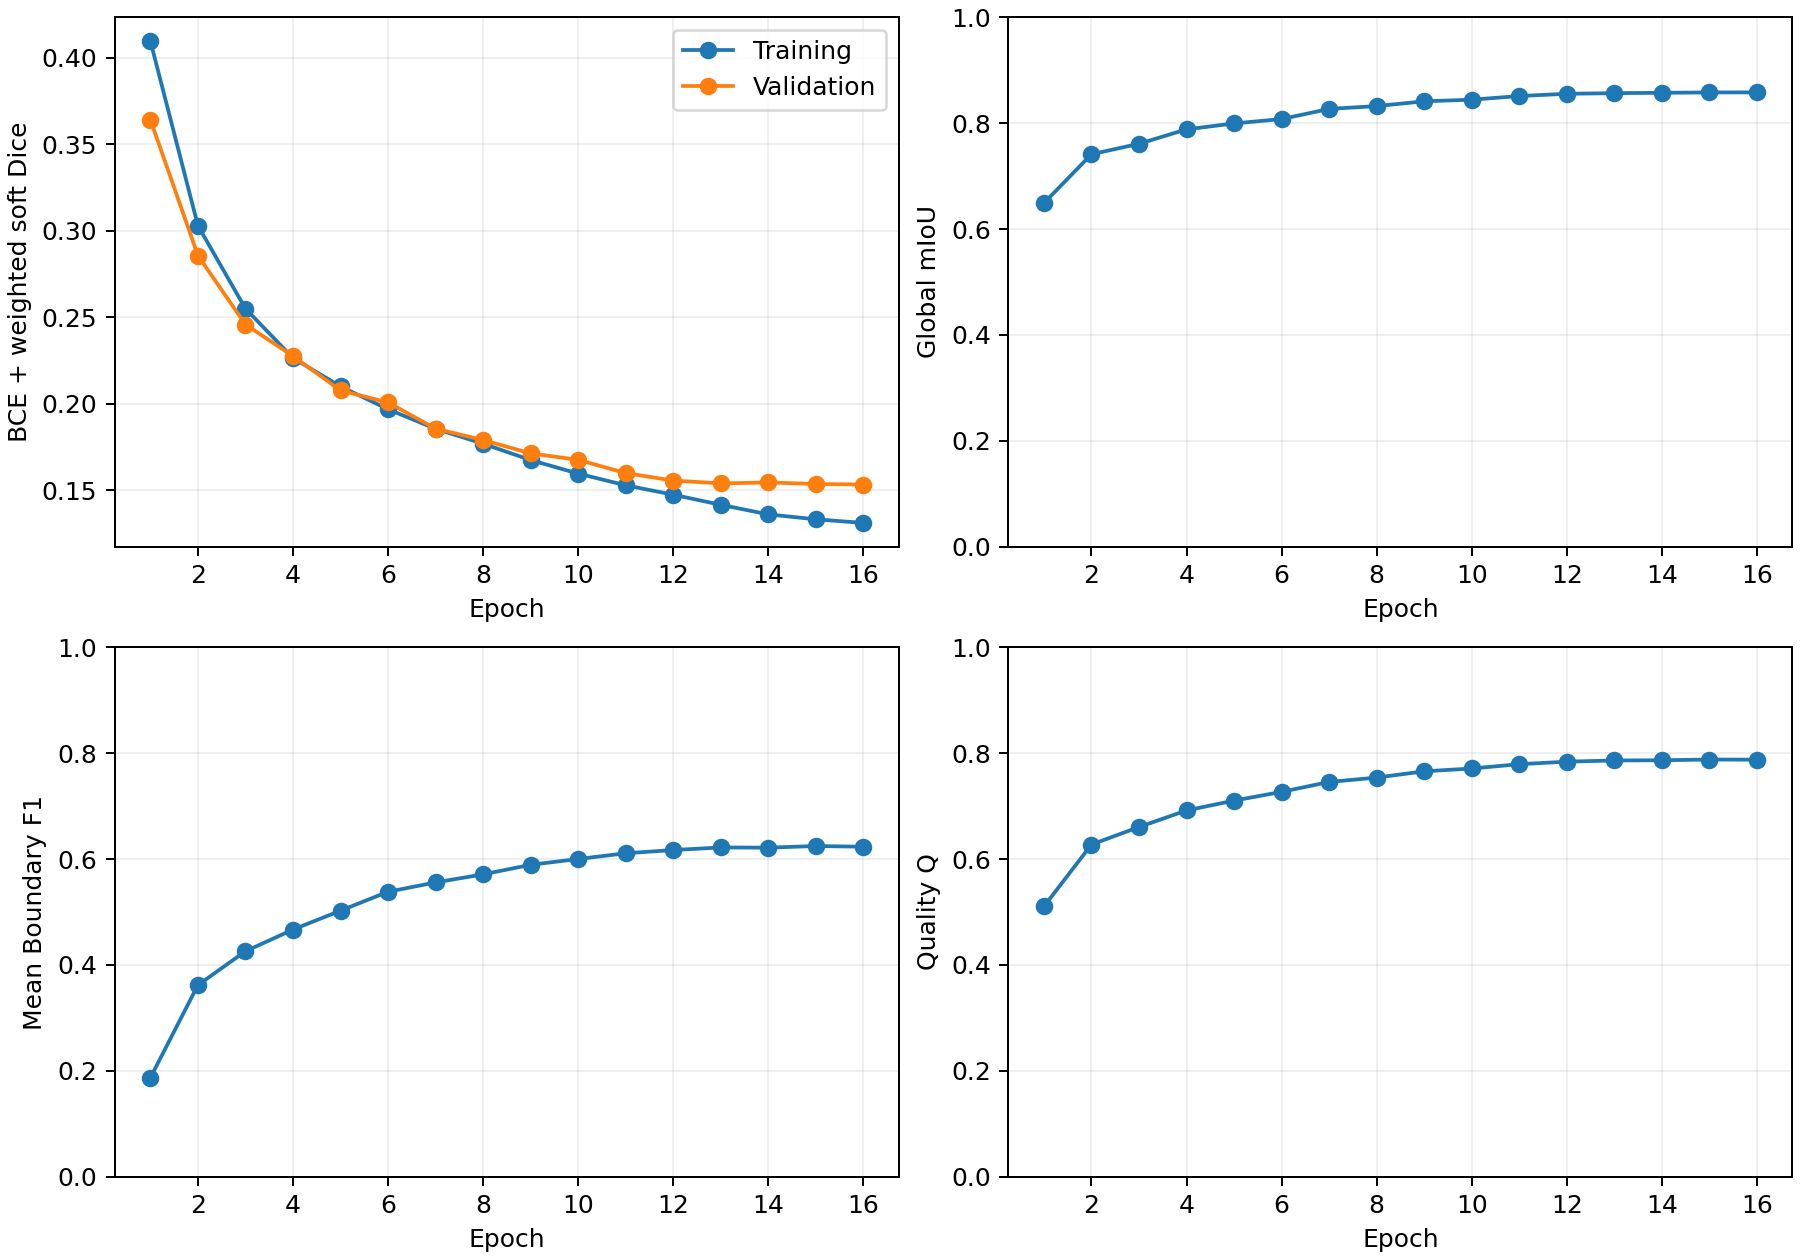
\includegraphics[width=\linewidth]{../results/figures/training.png}\caption{Actual recorded training and validation curves for the selected run.}\end{figure}}{}

\section{Results}
\begin{table}[htbp]\centering\small
\resizebox{\linewidth}{!}{\begin{tabular}{lrrrrrrr}
\toprule
Set & mIoU & BF1 & Q & CPU ms & Bytes & CES & $N$ \\
\midrule
Validation & 0.8591 & 0.6284 & 0.7899 & 24.319 & 1787043 & 0.6794 & 1055 \\
DUTS-TE & 0.7144 & 0.4441 & 0.6333 & 17.141 & 1787043 & 0.5629 & 5019 \\
Captured photos & 0.6226 & 0.3238 & 0.5329 & 14.063 & 1787043 & 0.4802 & 10 \\
\bottomrule
\end{tabular}
}
\caption{Evidence-derived results. Each row's time is measured on that set; storage is shared for the same checkpoint. Validation CES is an estimate; DUTS-TE CES is official only after all 5,019 images are evaluated. Missing evidence is reported as not evaluated.}
\end{table}
CPU and saved split information: Intel(R) Core(TM) 7 150U. Actual saved split: 9498 training and 1055 validation images; seed 42. Timing compliance must be assessed from the complete DUTS-TE row, not a short synthetic benchmark or an individual prediction.

\section{Captured-photo results}
No genuine captured photographs or annotations have been supplied. Evaluation and mandatory overlays remain incomplete.
All captures must appear, including unsuccessful cases. Annotation records document objects, lighting, distance, clutter, occlusion and manual annotation method. Ground truth and predictions are shown with the same green foreground and opacity $0.45$ over the corresponding image.

\section{Failure analysis}
\IfFileExists{failure_analysis.tex}{\section{Failure analysis}
The two lowest-scoring photos in Table~\ref{tab:cap} are the two failure cases (Figures~\ref{fig:ov1} and~\ref{fig:ov2}).
\begin{itemize}
\item \textbf{Clutter and many similar objects} (\texttt{cycle\_inside}, $Q=0.333$, BF1 $0.078$). The ground truth marks only the large bicycle in the right foreground, but the shed contains a whole row of bicycles. The network instead fires on the dense group of bicycles in the background and largely misses the foreground one. The task has no notion of ``the object the user means''; DUTS teaches saliency as a high-contrast, centred object, and with many equal candidates a small network with little global context picks the textured cluster. The same pattern lowers \texttt{study\_table} ($Q=0.369$) and \texttt{chair\_study-table}.
\item \textbf{Low-contrast, irregular object} (\texttt{outside\_plant}, $Q=0.365$, BF1 $0.108$). The ground truth is the row of shrubs, which resemble the soil and weeds in colour and texture. The prediction misses the shrubs and instead selects the bright concrete footpath. Foliage boundaries are thin and ragged, so even where overlap is acceptable the contour score is very low.
\end{itemize}
A milder issue is bleeding onto the supporting surface or neighbouring structure (\texttt{shoes}, \texttt{dustbin}: a small spur near the wall), probably because object and support share edges and colour statistics. The best case is the isolated, high-contrast \texttt{dustbin} ($Q=0.854$). Because the ground-truth masks are AI-generated references, part of the remaining error in any photo may come from the reference rather than the model.
}{At least two genuine failure explanations remain pending evaluated-image review. The visualization utility ranks actual observed examples by per-image quality to suggest candidates; a low score alone does not establish its cause. No lighting, occlusion, clutter or small-object failure is claimed without inspecting the relevant photo and mask.}

\section{Conclusion and limitations}
The implementation provides an auditable route from deterministic data preparation to trained parameter export and shared CPU evaluation. Architecture complexity is justified only by measured validation performance. Final segmentation quality, the full CPU budget, captured-photo generalization and submission completeness depend on the evidence in the results table. Pending entries prevent a submission-ready claim.

\clearpage
\section{Reproducibility}
Run these PowerShell commands in an outputs-empty copy containing source, configurations and genuine input data. Existing submitted weights/results should be preserved in a separate copy. Backticks continue a command on the next line. The complete selected configuration is \path{configs/final.json}; the single ``fixed'' trial below reproduces that configuration without searching against either test set. Original comparison/sweep commands are documented in the root README and \path{docs/REPRODUCIBILITY.md}.
{\small
\begin{verbatim}
python -m pip install -r requirements.txt
python -m scripts.verify
python -m scripts.download_duts --split TR
python -m scripts.prepare_dataset --root data/DUTS
python train.py --config configs/final.json --out experiments/reproduce/fixed
# Reuses that completed run, evaluates validation and records selection:
python -m scripts.run_experiments --config configs/final.json `
  --experiments configs/reproduce_experiments.json --out experiments/reproduce
python -m scripts.freeze_model
$tr = 'data/DUTS/DUTS-TR'
python evaluate.py --split validation --images "$tr/DUTS-TR-Image" `
  --masks "$tr/DUTS-TR-Mask" --manifest data/splits/val.txt `
  --out results/validation_metrics.json
python -m scripts.download_duts --split TE
$te = 'data/DUTS/DUTS-TE'
# This is both official quality evaluation and CPU timing:
python benchmark.py --split duts-test --images "$te/DUTS-TE-Image" `
  --masks "$te/DUTS-TE-Mask" --out results/duts_test_metrics.json
python predict.py --image photo.jpg --out mask.png
# Only after authentic capture and manual annotation:
python -m scripts.verify_dataset --root captured --split captured
python evaluate.py --split captured --images captured/images_256 `
  --masks captured/masks_256 --out results/captured_metrics.json
python -m scripts.create_figures overlays `
  --images captured/images_256 --masks captured/masks_256 `
  --out results/captured_figures
python -m scripts.create_figures comparison
python -m scripts.build_report
python -m scripts.audit --submission
python -m scripts.package_submission
\end{verbatim}}
Prediction loads \path{weights/final_model.pth} and prints exactly \texttt{T\_CPU\_ms:} and \texttt{S\_disk\_bytes:}. The first pass writes the mask; the next 20 passes are timed. Report building supports pdflatex or an explicitly supplied portable Tectonic executable. Every compiled page requires visual review. Unavailable captured-photo evidence prevents the final audit from passing, even if all software tests pass.

\begin{thebibliography}{9}
\small
\setlength{\itemsep}{0pt}
\bibitem{assignment} CSL7360, \emph{Assignment 2: Cost-Efficient Segmentation under a Compute Budget}, supplied assignment PDF, pp. 1--3.
\bibitem{duts} L. Wang et al., \emph{Learning to Detect Salient Objects with Image-level Supervision}, CVPR, 2017. Dataset: \url{https://saliencydetection.net/duts/}.
\end{thebibliography}
\end{document}
